\documentclass[a4paper,12pt]{article}

\usepackage{mystyle}
\usepackage{gensymb}

\graphicspath{ {images/} }

\usetikzlibrary{arrows.meta}

\definecolor{my-red}{RGB}{176, 0, 0}
\definecolor{my-blue}{RGB}{0, 0, 153}

% \newcommand{\eps}{\epsilon}


% https://tex.stackexchange.com/a/4817/135045
\makeatletter
\newcommand*{\Relbarfill@}{\arrowfill@\Relbar\Relbar\Relbar}
\newcommand*{\xeq}[2][]{\ext@arrow 0055\Relbarfill@{#1}{#2}}
\makeatother


\author{Алексеев Василий}

\title{Семинар 7}
\date{20 + 24 октября 2022}


\begin{document}
  \maketitle
  
  \tableofcontents

  \thispagestyle{empty}
  
  \newpage
  
  \pagenumbering{arabic}


  \section{Кривые второго порядка}
  
  Прямая в общей декартовой системе координат (ОДСК) на плоскости задавалась линейным уравнением:
  \[
    Ax + By + C = 0,\quad A^2 + B^2 > 0
  \]
  
  Кривая \emph{второго} порядка в ОДСК на плоскости задаётся уравнением вида:
  \[
    \boxed{
      \left\{
        \begin{aligned}
          &Ax^2 + 2Bxy + Cy^2 + 2Dx + 2Ey + F = 0\\
          &A^2 + B^2 + C^2 > 0
        \end{aligned}
      \right.
    }
  \]
  
  Всего существует несколько ``типов'' кривых второго порядка.
  Рассмотрим далее самые ``популярные''.
  
  
  \subsection{Эллипс}
  
  \begin{definition}
    \emph{Эллипсом} называется такая кривая второго порядка, которая в некоторой декартовой прямоугольной системе координат (ДПСК) может быть задана уравнением вида:
    \begin{equation}\label{eq:ellipse}
      \boxed{
        \left\{
          \begin{aligned}
            &\frac{x^2}{a^2} + \frac{y^2}{b^2} = 1\\
            &a \geq b > 0
          \end{aligned}
        \right.
      }
    \end{equation}
    
    Указанная система координат называется \emph{канонической системой координат}, а уравнение эллипса~(\ref{eq:ellipse}) в этой системе координат~---~\emph{каноническим уравнением} эллипса.
  \end{definition}
  
  По уравнению (\ref{eq:ellipse}) можно видеть, что эллипс ограничен.
  Причём ``крайние'' точки~---~это точки с координатами $(\pm a, 0)$ и $(0, \pm b)$.
  Эти точки называются \emph{вершинами} эллипса.
  Величины $a$ и $b$~---~это \emph{большая и малая полуоси} эллипса соответственно (см. рисунок~(\ref{fig:ellipse})).
  С эллипсом связаны ещё две особые точки~---~\emph{фокусы} эллипса.
  Фокусы~---~это точки $F_1(c, 0)$ и $F_2(-c, 0)$, где $c$~---\emph{фокальное расстояние} и считается для эллипса по формуле:
  \begin{equation}\label{eq:ellipse-c}
    c = \sqrt{a^2 - b^2}
  \end{equation}
  
  \begin{figure}[h]
    \centering
    
    \includegraphics[width=0.8\textwidth]{ellipse}
    
    \caption{Эллипс и ``всё основное'', что с ним связано.}
    \label{fig:ellipse}
  \end{figure}
  
  \emph{Эксцентриситетом} эллипса $\eps$ называется следующая величина:
  \begin{equation}
    \eps = \frac{c}{a}
  \end{equation}
  
  Из~(\ref{eq:ellipse-c}) видно, что $\eps \hm< 1$.
  Также очевидно, что $\eps \hm> 0$.
  При этом возможен и случай $\eps \hm= 0$, когда $a \hm= b$, то есть для окружности.
  
  Выделяются две прямые, называемые \emph{директрисами} эллипса:
  \[
    d_1\colon x = \frac{a}{\eps},\quad d_2\colon x = -\frac{a}{\eps}
  \]
  
  \medskip
  
  Выясним, что ``интересного'' связано с введёнными ``буквами'' и понятиями.
  
  Оказывается, что \emph{сумма расстояний от произвольной точки эллипса до фокусов постоянна}.
  Проверим это.
  Пусть точка $M(x_0, y_0)$ лежит на эллипсе, то есть её координаты удовлетворяют соотношению:
  \begin{equation}\label{eq:m-on-the-ellipse}
    \frac{x_0^2}{a^2} + \frac{y_0^2}{b^2} = 1
  \end{equation}
  Найдём расстояние $|MF_1|$ от точки $M$ до фокуса $F_1$.
  Обозначим это расстояние как $r_1$~---~один из двух \emph{фокальных радиусов} точки $M$.
  Так как система координат прямоугольная, то $r_1$ можно посчитать по формуле:
  \[
    r_1 = \sqrt{(x_0 - c)^2 + y_0^2}
  \]
  
  Выразим $y_0$ из соотношения для координат точки $M$~(\ref{eq:m-on-the-ellipse}), подставим в формулу для $r_1$ и проведём ещё несколько несложных преобразований и ``переименований'':
  \begin{equation}
  \begin{split}
    r_1 = \sqrt{(x_0 - c)^2 + y_0^2}
        = \sqrt{(x_0 - c)^2 + b^2\left(1 - \frac{x_0^2}{a^2}\right)}
        = \ldots
        = a - \eps x_0
  \end{split}
  \end{equation}
  
  Аналогичным образом можно получить, что расстояние $|MF_2|$ от точки $M$ до второго фокуса $F_2$ выражается как:
  \[
    r_2 = a + \eps x_0
  \]
  
  Складывая фокальные радиусы, получаем:
  \begin{equation}\label{eq:ellipse-r1-plus-r2}
    \boxed{
        r_1 + r_2 = 2a
    }
  \end{equation}
  
  То есть сумма расстояний от точки эллипса до фокусов в самом деле постоянна, причём равна $2a$.
  Но верно также и \emph{обратное} свойство.
  Пусть даны $a \hm\geq b \hm> 0$.
  Пусть выбраны две точки с координатами $(\pm c, 0)$, где $c \hm= \sqrt{a^2 \hm- b^2}$.
  Тогда если про некоторое множество точек $\mathcal P$ известно, что для точек из $\mathcal P$ и только для таких точек верно, что сумма расстояний от точки до двух заранее выбранных $(\pm c, 0)$ постоянна и равна $2a$, то $\mathcal P$ есть эллипс.
  
  Проверим.
  Выберем точку $M(x_0, y_0)$ из описанного множества точек $\mathcal P$ и распишем сумму расстояний от неё до двух фиксированных точек:
  \[
    \sqrt{(x_0 - c)^2 + y_0^2} + \sqrt{(x_0 + c)^2 + y_0^2} = 2a
  \]
  
  Избавляясь от корней (например, возводя два раза в квадрат обе части равенства), получаем соотношение:
  \[
    \frac{x_0^2}{a^2} + \frac{y_0^2}{b^2} = 1
  \]
  
  То есть произвольная точка из $\mathcal P$ лежит на эллипсе с большой полуосью $a$, малой $b$ и фокусами $(\pm c, 0)$.
  И при этом нет таких точек, которые бы были на указанном эллипсе, но не были бы в $\mathcal P$.
  Таким образом, $\mathcal P$ и есть эллипс. \qed
  
  \medskip
  
  С директрисами связано следующее свойство.
  \emph{Отношение расстояния от точки $M(x_0, y_0)$ эллипса до фокуса к расстоянию от $M$ до соответственной директрисы равно эксцентриситету $\eps$}.
  Например, для расстояний до фокуса $F_1$ и директрисы $d_1$:
  \[
    \frac{r_1}{\rho(M, d_1)} = \frac{a - \eps x}{a/\eps - x} = \eps
  \]
  
  
  \subsection{\# 7.25(5)}
  
  В данной системе координат эллипс имеет каноническое уравнение.
  Составить это уравнение, если расстояние от директрисы до ближайшей вершины равно $4$.
  А до вершины, лежащей на оси $OY$, расстояние равно $8$.
  
  \begin{solution}
    Перепишем условие ``в нужных терминах''.
    
    Расстояние от директрисы до ближайшей вершины:
    \[
      a/\eps - a = 4
    \]
    
    Расстояние от директрисы до вершины на $OY$:
    \[
      a/\eps - 0 = 8
    \]
    
    Получается, $a \hm= 4$, $\eps \hm= 1/2 \hm< 1$.
    Теперь можно найти малую полуось:
    \[
      \left\{
        \begin{aligned}
          &\eps = c / a\\
          &c^2 = a^2 - b^2
        \end{aligned}
      \right. \Rightarrow b^2 = a^2 (1 - \eps^2) =  4^2 (1 - (1/2)^2) = 12
    \]
    
    Можем выписать каноническое уравнение:
    \[
      \frac{x^2}{16} + \frac{y^2}{12} = 1
    \]
  \end{solution}
  
  
  \subsection{\# 7.26(4)}
  
  Вычислить эксцентриситет эллипса, если отрезок между фокусами виден из конца малой оси под прямым углом.
  
  \begin{solution}
    Пусть $B$~---~``верхняя'' вершина эллипса (один из концов малой оси).
    Тогда треугольник $\triangle BF_1F_2$ по условию прямоугольный.
    Очевидно, он также и равнобедренный: $BF_1 \hm= BF_2 \hm\equiv r_b$.
    
    Сумма расстояний от точки эллипса до фокусов постоянна и равна $2a$~(\ref{eq:ellipse-r1-plus-r2}).
    В случае с точкой $B$ это значит, что $BF_1 \hm+ BF_2 \hm= 2a \hm\Rightarrow r_b \hm= a$.
    
    Вернёмся к треугольнику $\triangle BF_1F_2$.
    Так как он прямоугольный:
    \[
      F_1F_2^2 = BF_1^2 + BF_2^2 \Leftrightarrow (2c)^2 = a^2 + a^2 
    \]
    
    Таким образом,
    \[
      c = \frac{a}{\sqrt{2}}
    \]
    
    И потому эксцентриситет эллипса оказывается равным:
    \[
      \eps = \frac{c}{a} = \frac{1}{\sqrt{2}}
    \]
  \end{solution}
  
  
  \subsection{Гипербола}
  
  \begin{definition}
    \emph{Гипербола}~---~кривая второго порядка, которая в некоторой декартовой прямоугольной системе координат может быть описана уравнением:
    \begin{equation}\label{eq:hyperbolical}
      \boxed{
        \frac{x^2}{a^2} - \frac{y^2}{b^2} = 1
      }\quad a > 0,\ b > 0
    \end{equation}
    
    Прямоугольная декартова система координат, в которой гипербола описывается уравнением вида~(\ref{eq:hyperbolical}), называется \emph{канонической}, и само уравнение~(\ref{eq:hyperbolical}) в таком случае~---~\emph{каноническим} уравнением гиперболы.
  \end{definition}
  
  По уравнению~(\ref{eq:hyperbolical}) можно видеть, что гипербола неограничена.
  Также видно, что, например, точки $(\pm a, 0)$ лежат на гиперболе.
  А ось $OY$ гипербола вообще никогда не пересекает...
  
  \begin{figure}[h]
    \centering
    
    \includegraphics[width=0.8\textwidth]{hyperbola}
    
    \caption{Гипербола и ``всё основное'', что с ней связано.}
    \label{fig:hyperbola}
  \end{figure}
  
  Оказывается, что у гиперболы есть две наклонных асимптоты (см. рисунок~(\ref{fig:hyperbola})):
  \[
    \boxed{
      y = \pm \frac{b}{a} x
    }
  \]
  Проверим, что это так.
  Если у гиперболы есть асимптота, то она будет ``пределом касательной'' в точке $M(x_0, y_0)$ при стремлении $x_0 \hm\to +\infty$.
  Найдём уравнение касательной к гиперболе в точке $M(x_0, y_0)$.
  Пусть, для определённости, $x_0 \hm> 0$ и $y_0 \hm> 0$.
  Будем искать уравнение касательной в виде:
  \[
    y = k_1 x + k_2
  \]

  Коэффициент $k_1$~---~тангенс угла наклона касательной к оси $OX$.
  На него можно смотреть как на предел
  \[
    k_1 = \lim_{x \to x_0} \frac{y - y_0}{x - x_0} = \lim_{dx \to 0} \left.\frac{dy}{dx}\right|_{x=x_0}
  \]
  
  Чтобы найти этот предел, можно сначала взять дифференциал от обеих частей уравнения гиперболы в точке $M(x_0, y_0)$:
  \[
    \frac{x_0 dx}{a^2} - \frac{y_0 dy}{b^2} = 0 \Rightarrow \left.\frac{dy}{dx}\right|_{x=x_0} = \frac{x_0 b^2}{y_0 a^2}
  \]
  
  Таким образом,
  \[
    k_1 = \frac{x_0 b^2}{y_0 a^2}
  \]
  
  \begin{figure}[h]
    \centering
    
    \includegraphics[width=0.8\textwidth]{hyperbolic_tangent_to_asymptote}
    
    \caption{Касательная к гиперболе в точке $(x_0, y_0)$, $x_0 \hm> 0$, $y_0 \hm> 0$ при увеличении $x_0$.}
    \label{fig:hyperbolic_tangent_to_asymptote}
  \end{figure}
  
  Как себя ведёт угол наклона касательной при $x_0 \hm\to +\infty$?
  Для определённости будем двигать точку касания ``выше'' оси $OX$, то есть считаем, что $y_0 \hm> 0$ (см. рисунок~(\ref{fig:hyperbolic_tangent_to_asymptote})).
  При нахождении предела $k_1$ воспользуемся тем, что точка касания лежит и на гиперболе~---~благодаря этому можно выразить $y_0$ через $x_0$:
  \[
    \lim_{x_0\to +\infty} k_1
      = \lim_{x_0\to +\infty} \frac{x_0 b^2}{y_0 a^2}
      = \lim_{x_0\to +\infty} \frac{x_0 b^2}{a^2 \sqrt{b^2 \left(\frac{x_0^2}{a^2} - 1\right)}}
      = \frac{b}{a}
  \]
  
  То есть у гиперболы в самом деле есть асимптота.
  Остаётся найти коэффициент $k_2$.
  Для касательной он будет равен:
  \[
    y_0 = k_1 x_0 + k_2 \Rightarrow k_2 = y_0 - k_1 x_0 = y_0 - \frac{x_0^2 b^2}{y_0 a^2} = -\frac{b^2}{y_0}
  \]
  
  И для асимптоты:
  \[
    \lim_{x_0\to +\infty} k_2
    = \lim_{x_0\to +\infty} -\frac{b^2}{y_0}
    = 0
  \]
  
  Мы рассматривали точки касания $(x_0, y_0)$, у которых $x_0 \hm> 0$ и $y_0 \hm> 0$.
  Такую же асимптоту получили бы и для точек из третьей координатной четверти.
  В других случаях (для точек гиперболы из второй и четвёртой четвертей) могли бы ещё получить асимптоту с углом наклона $-b/a$.
  
  \medskip
  
  Итак, гипербола состоит из двух ветвей.
  Точки $(\pm a, 0)$ называются \emph{вершинами} гиперболы.
  Величина $a$ называется \emph{действительной полуосью}, а $b$~---~\emph{мнимой полуосью}.
  У гиперболы, так же, как и у эллипса, есть два фокуса~---~точки с координатами $F_1(c, 0)$ и $F_2(-c, 0)$.
  Правда, \emph{фокальное расстояние} $c$ считается уже по-другому:
  \[
    \boxed{
      c = \sqrt{a^2 + b^2}
    }
  \]
  Таким образом, у гиперболы $c \hm> a$.
  
  Далее, у гиперболы, так же, как и у эллипса, есть \emph{эксцентриситет}, который определяется как отношение:
  \[
    \eps = \frac{c}{a}
  \]
  Как видно из формулы, эксцентриситет гиперболы \emph{больше единицы}.
  
  Определим также две вертикальные прямые~---~\emph{директрисы} гиперболы:
  \[
    d_1\colon x = \frac{a}{\eps},\quad d_2\colon x = -\frac{a}{\eps}
  \]
  
  Аналогично случаю с эллипсом, можно получить формулы для расстояния от точки гиперболы $M(x_0, y_0)$ до фокусов $F_1$ и $F_2$:
  \[
    r_1 = |MF_1| = |a - \eps x_0|,\quad r_2 = |MF_2| = |a + \eps x_0|
  \]
  
  Модули уже будут раскрываться по-разному для точек из разных координатных четвертей.
  Но можно убедиться в том, что во всех случаях \emph{модуль разности расстояний от точки гиперболы до фокусов постоянен}:
  \[
    \boxed{
      |r_1 - r_2| = 2a
    }
  \]
  
  Также несложно проверить, что \emph{отношение расстояния от точки гиперболы $M$ до фокуса к расстоянию от $M$ до соответственной директрисы равно эксцентриситету}:
  \[
    \frac{r_1}{\rho(M, d_1)} = \eps
  \]
  
  
  \subsection{\# 7.38(4)}
  
  В данной системе координат гипербола имеет каноническое уравнение.
  Составить это уравнение, если длина мнимой полуоси равна $1$, а вершина гиперболы делит отрезок между фокусами в отношении $4 \hm: 1$.
  
  \begin{solution}
    Снова попытаемся ``переписать условие'', но на этот раз ``в терминах гиперболы''.
    Получается, дана длина мнимой полуоси: $b \hm= 1$.
    До канонического уравнения не хватает найти $a$.
    
    Отношение длин отрезков, на которые вершина делит отрезок между фокусами:
    \[
      \frac{c + a}{c - a} = \frac{4}{1} \Rightarrow 5a = 3c
    \]
    
    Выразим $c$ через $a$ и $b$:
    \[
      c^2 = a^2 + b^2 = a^2 + 1
    \]
    
    Возведём в квадрат соотношение, полученное шагом ранее, и подставим выражение для $c$:
    \[
      25 a^2 = 9 (a^2 + 1) \Rightarrow a = 3/4
    \]
    
    Тогда каноническое уравнение:
    \[
      \frac{16}{9}x^2 - y^2 = 1
    \]
  \end{solution}
  
  
  \subsection{\# 7.40(2)}
  
  Вычислить эксцентриситет гиперболы, если угол между асимптотами, содержащий фокус, равен $120\degree$.
  
  \begin{solution}
    Половина угла между асимптотами есть $60\degree$.
    Таким образом, тангенс угла наклона асимптоты:
    \[
      \frac{b}{a} = \tg{60\degree} = \sqrt{3}
    \]
    
    Эксцентриситет гиперболы:
    \[
      \eps = \frac{c}{a} = \frac{\sqrt{a^2 + b^2}}{a}
      = \sqrt{1 + \left(\frac{b}{a}\right)^2}
      = 2 > 1
    \]
  \end{solution}
  
  
  \subsection{Парабола}
  
  \begin{definition}
    \emph{Параболой} называется кривая второго порядка, которая в некоторой декартовой прямоугольной системе координат может быть задана уравнением вида:
    \begin{equation}\label{eq:parabolical}
      \boxed{y^2 = 2px}\quad p > 0
    \end{equation}
    
    Декартова прямоугольная система координат, где парабола задаётся уравнением вида~(\ref{eq:parabolical}), называется \emph{канонической системой координат}, а само уравнение параболы в этой системе координат~---~\emph{каноническим уравнением} параболы.
  \end{definition}
  
  \begin{figure}[h]
    \centering
    
    \includegraphics[width=0.8\textwidth]{parabola}
    
    \caption{Парабола и ``всё основное'', что с ней связано.}
    \label{fig:parabola}
  \end{figure}
  
  Видно, что, парабола неограничена.
  Также видно, что, в отличие от рассмотренных ранее эллипса~(\ref{eq:ellipse}) и гиперболы~(\ref{eq:hyperbolical}), парабола имеет только одну ось симметрии (см. рисунок~(\ref{fig:parabola})): если точка $(x_0, y_0)$ лежит на параболе, то и точка $(x_0, -y_0)$ лежит на ней, но у всех точек параболы $x_0 \hm> 0$.
  
  Величина $p$ называется \emph{параметром параболы}.
  \emph{Фокус} параболы~---~точка $F(p/2, 0)$.
  Директриса~---~вертикальная прямая
  $
    d\colon x \hm= -p/2
  $.
  Эксцентриситет параболы полагается равным единице:
  $
    \eps = 1
  $.
  
  Найдём расстояние от точки $M(x_0, y_0)$ параболы до фокуса $F$:
  \[
    r = \sqrt{(x_0 - p/2)^2 + y_0^2} \xeq{y_0^2 = 2px_0} x_0 + p/2
  \]
  
  Видно, что \emph{отношение расстояния от точки $M(x_0, y_0)$ параболы до фокуса к расстоянию от $M$ до директрисы равно эксцентриситету $\eps$} (то есть указанные расстояния одинаковые):
  \[
    \frac{r}{\rho(M, d)} = \frac{x_0 + p/2}{x_0 - (-p/2)} = 1 = \eps
  \]
  
  
  \subsection{\# 7.54(3)}
  
  В данной системе координат парабола имеет каноническое уравнение.
  Составить это уравнение, если длина хорды, проходящей через фокус под углом $45\degree$ к оси параболы, равна $18$.
  
  \begin{solution}
    Не совсем очевидно\footnote{По крайней мере, автору конспекта не очевидно :)}, можно ли как-то ``по-простому'', как в аналогичных номерах для эллипса и гиперболы, переписать условие в нужных терминах, чтобы сразу что-то посчитать...
    Поэтому предлагается пойти, возможно не самым оптимальным, но точно ``пробивным'' путём.
    Найдём уравнение прямой $l$, содержащей описанную хорду.
    Определим точки~---~концы хорды.
    И после этого составим уравнение, используя данную в условии длину хорды.
    
    Будем искать уравнение прямой $l$ в виде $y \hm= ax \hm+ b$ (наклонная прямая).
    Нам дан угол наклона хорды, поэтому сразу понятно, что $a \hm= 1$.
    Далее, прямая $l$ проходит через фокус, поэтому можно записать:
    \[
      0 = \frac{p}{2} + b \Rightarrow b = -\frac{p}{2}
    \]
    
    Таким образом, уравнение прямой $l$, которая содержит хорду из условия:
    \[
      y = x - \frac{p}{2}
    \]
    
    Теперь определим точки пересечения прямой $l$ и параболы (концы хорды):
    \[
      \left\{
        \begin{aligned}
          &y^2 = 2px\\
          &y = x - \frac{p}{2}
        \end{aligned}
      \right.
    \]
    
    Решая систему, находим координаты точек:
    \[
      \left\{
        \begin{aligned}
          &x = \frac{3p \pm 2p\sqrt{2}}{2}\\
          &y = 2p \pm 2p\sqrt{2}
        \end{aligned}
      \right.
    \]
    
    Длина хорды:
    \[
      18^2 = \left(\frac{3p + 2p\sqrt{2}}{2} - \frac{3p - 2p\sqrt{2}}{2}\right)^2
             + \Biggl(\left(2p + 2p\sqrt{2}\right) - \left(2p - 2p\sqrt{2}\right)\Biggr)^2
           \Rightarrow p = \frac{9}{2}
    \]
    
    И потому каноническое уравнение параболы:
    \[
      y^2 = 9x
    \]
  \end{solution}
  
  
  \newpage
  
  
  \section{Дополнение}
  
  \subsection{Про конические сечения}
  
  Кривые второго порядка можно получать, пересекая двойной круговой конус (не обязательно прямой) плоскостью, не проходящей через вершину конуса (\ref{fig:conic_sections}).
  
  \begin{figure}[h]
    \centering
    
    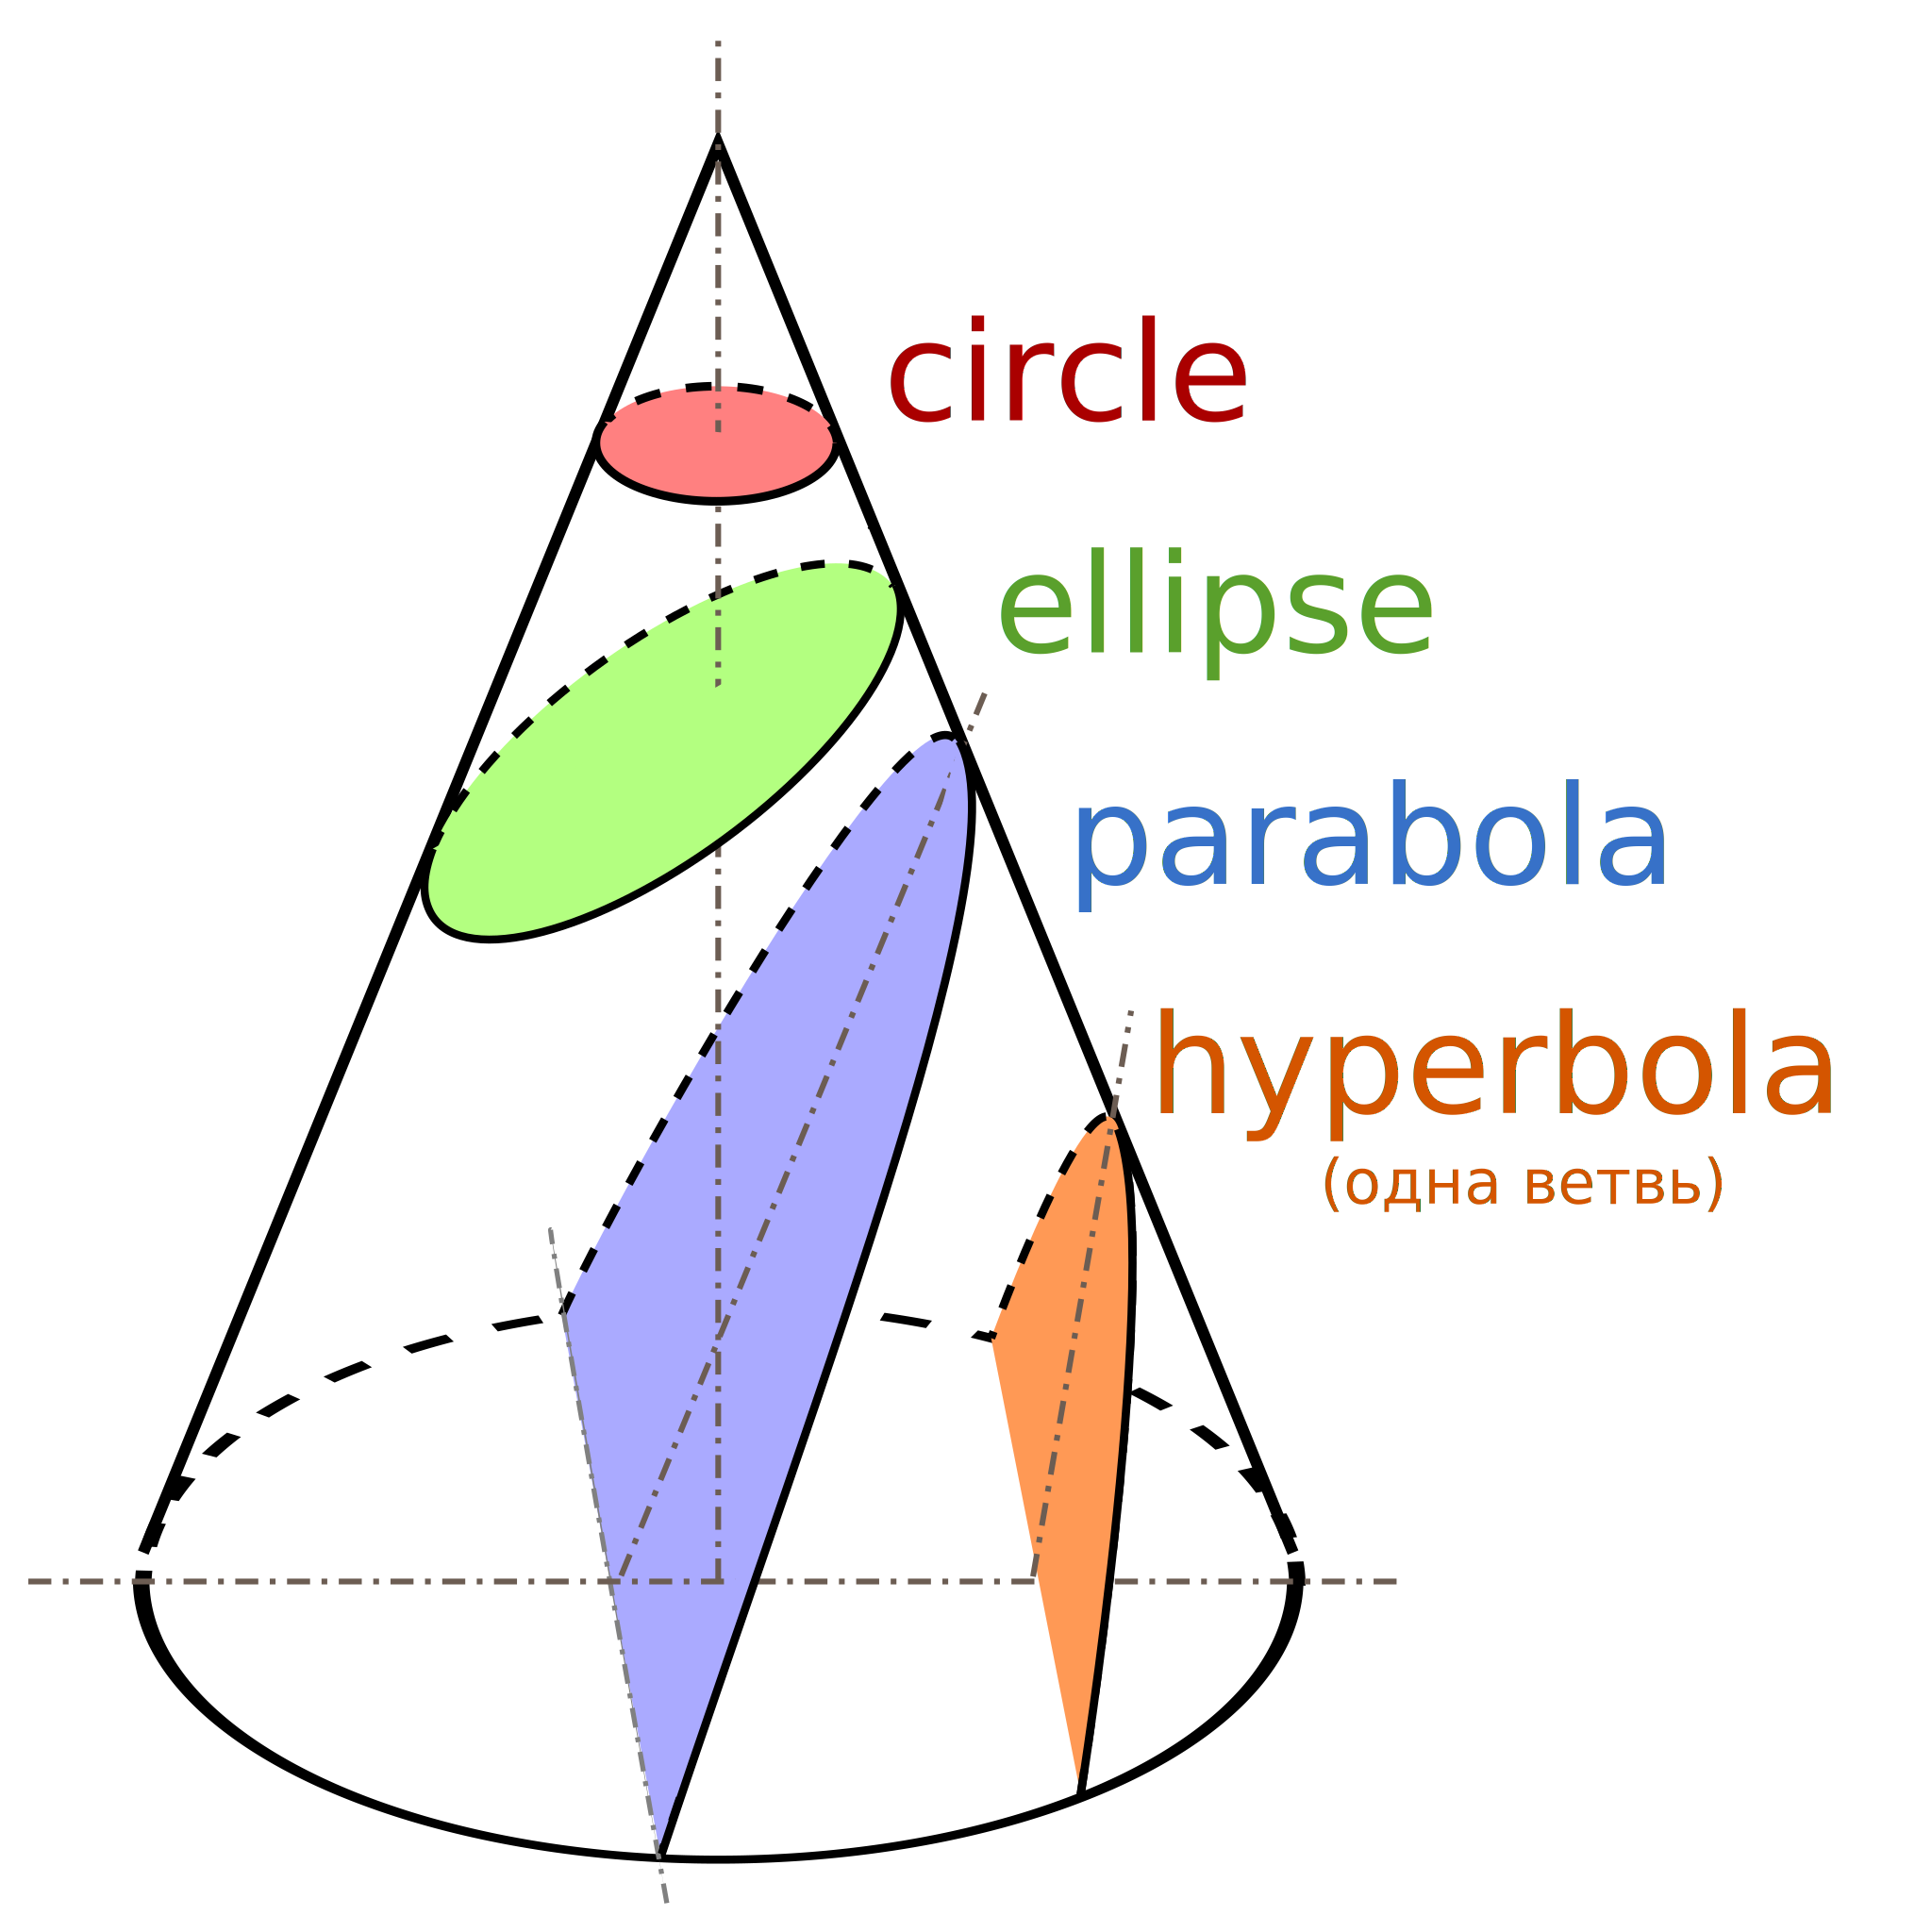
\includegraphics[width=0.4\textwidth]{conic_sections}
    
    \caption{Кривые второго порядка (эллипс, гипербола и парабола)~---~\href{https://en.wikipedia.org/wiki/Conic_section}{как конические сечения}.}
    \label{fig:conic_sections}
  \end{figure}
  
  Можно заметить, что эксцентриситет увеличивается в ряду ``окружность -- эллипс -- парабола -- гипербола'' (\ref{fig:eccentricity}).
  Таким образом, эксцентриситет выражает некую меру кривизны кривой: от максимальной у окружности до минимальной у гиперболы.

  \begin{figure}[h]
    \centering
    
    \begin{minipage}[c]{0.4\textwidth}  % https://tex.stackexchange.com/a/29163/135045
      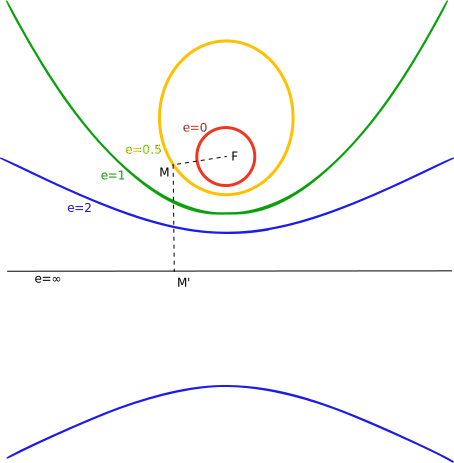
\includegraphics[width=\textwidth]{eccentricity}
    \end{minipage}\hfill
    \begin{minipage}[c]{0.55\textwidth}
      \caption{Эксцентриситет~---~как число, \href{https://en.wikipedia.org/wiki/Conic_section}{отражающее кривизну линии второго порядка}. Кривизна уменьшается с увеличением эксцентриситета.}
      \label{fig:eccentricity}
    \end{minipage}
  \end{figure}
  
  
  Мы определяли эксцентриситет для эллипса и гиперболы через отношение $c$ к $a$ (к слову,  $c$ ещё называют \emph{линейным эксцентриситетом} или \emph{фокальным расстоянием}~---~расстояние между центром и фокусом).
  У параболы же нет $c$ (так как нет центра), но отношение расстояния от точки параболы до фокуса к расстоянию от той же точки до директрисы было равно $1$, то есть эксцентриситету параболы...
  Существует более общее определение эксцентриситета, которое подходит как для окружности, так и для эллипса, гиперболы и параболы~---~через конические сечения (\ref{fig:eccentricity_definition}):
  \[
    \left\{
      \begin{aligned}
        &\eps = \frac{\sin \beta}{\sin \alpha}\\
        &0 < \alpha < \frac{\pi}{2}\\
        &0 \leq \beta \leq \frac{\pi}{2}
      \end{aligned}
    \right.
  \]
  где $\beta$~---~угол наклона секущей конус плоскости, а $\alpha$~---~угол между образующей конуса и его основанием.
  
  В пределе $\alpha \hm\to +0$ (сплющенный конус) в сечении в пределе получается прямая, поэтому для прямой можно считать эксцентриситет $\eps \hm\to +\infty$ (\ref{fig:eccentricity}).
  
  
  \begin{figure}[h]
    \centering
    
    \begin{minipage}[c]{0.25\textwidth}
      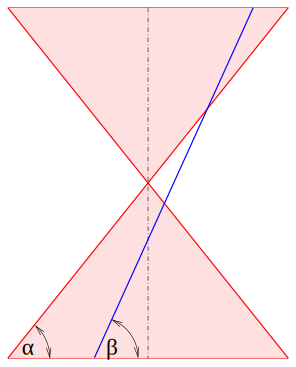
\includegraphics[width=\textwidth]{eccentricity_definition}
    \end{minipage}\hfill
    \begin{minipage}[c]{0.75\textwidth}
      \caption{К определению \href{https://en.wikipedia.org/wiki/Eccentricity_(mathematics)}{эксцентриситета через конические сечения}.}
      \label{fig:eccentricity_definition}
    \end{minipage}
  \end{figure}
  
  
  \subsection{Про $2p$}
  
  В каноническом уравнении параболы
  \[
    y^2 = 2px,\quad p > 0
  \]
  двойка на самом деле ``не просто так'': $p$~---~половина так называемого \emph{latus rectum}\footnote{Latus переводится с латинского как ``прямой'', а rectum~---~``кишка''?.. Или это всё вместе переводится как ``прямая сторона'' (по другим источникам)?.. Автору конспекта ответ не известен.} (\ref{fig:semi_latus_rectum}).
  То есть $p$~---~это длина части перпендикуляра к оси параболы, проходящего через фокус, от фокуса до параболы.
  Точно так же $p$ определяется и в случае эллипса и гиперболы.
  
  \begin{figure}[h]
    \centering

    \begin{minipage}[c]{0.4\textwidth}
      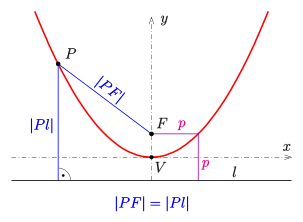
\includegraphics[width=\textwidth]{semi_latus_rectum}
    \end{minipage}\hfill
    \begin{minipage}[c]{0.55\textwidth}
      \caption{Число $p$ из \href{https://en.wikipedia.org/wiki/Parabola}{канонического уравнения параболы}.}
      \label{fig:semi_latus_rectum}
    \end{minipage}
  \end{figure}
\end{document}
